\begin{figure}[ht]
    \centering
    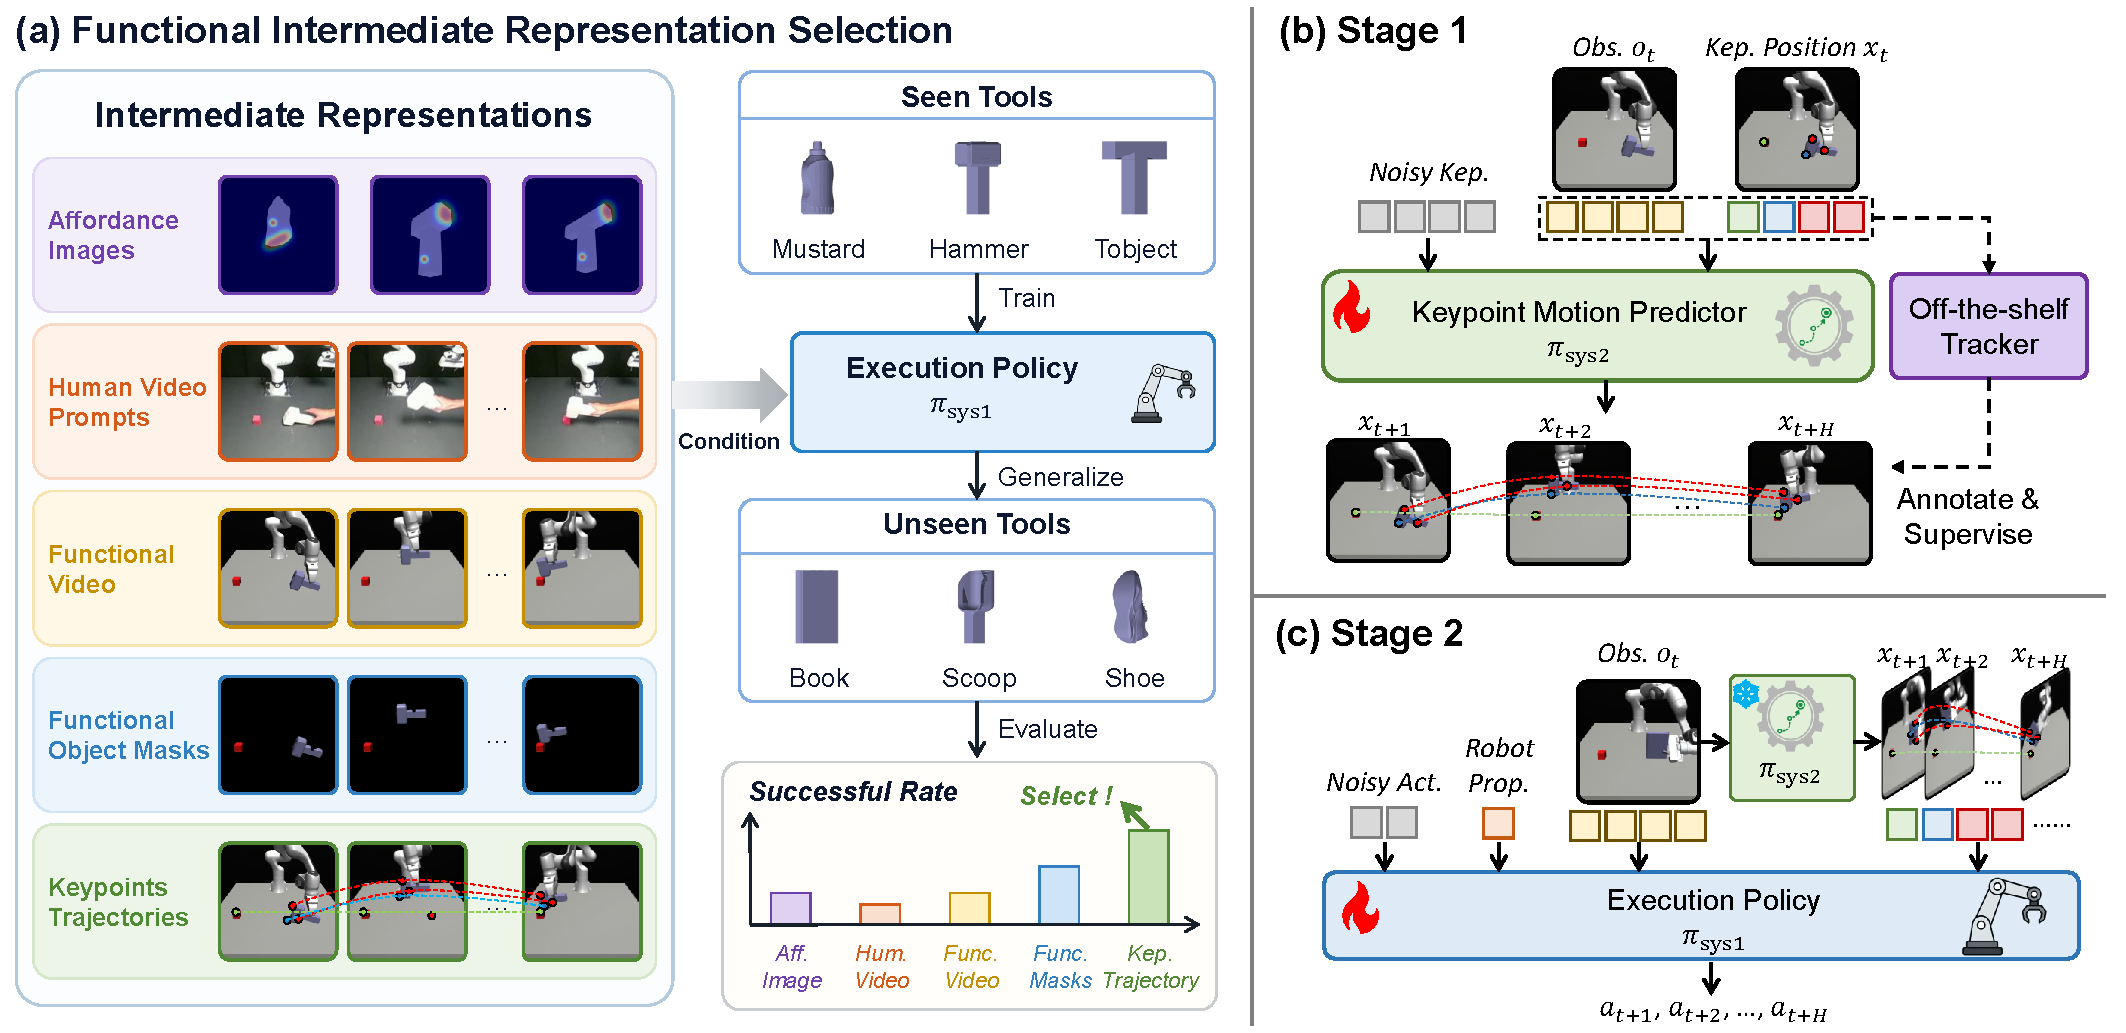
\includegraphics[width=0.95\linewidth]{figures/main_pipeline_v2.pdf}
    \caption{
    \textbf{Overview of the \algoname{}.} (a) Evaluation and selection of functional intermediate representations. (b) In Stage 1, the System-2 planner learns to predict future keypoint-based functional plans from action-free observations. (c) In Stage 2, the System-1 execution policy grounds the predicted functional plans into executable robot actions.
    }
    \label{fig:functional_generalization_pipeline}
\end{figure}

\vspace{-15pt}
\section{Methods}
\label{sec:method}



\subsection{Problem Formulation}
We formulate functional generalization in tool-use manipulation as a Markov Decision Process (MDP), where the state $\mathbf{s}_t$ consists of the visual observation $\mathbf{o}_t$, the proprioceptive state $\mathbf{q}_t$, and optionally a functional intermediate representation $\mathbf{x}_t$ (e.g., keypoint trajectories) that carries function-relevant cues bridging perception and action, and the action $\mathbf{a}_t$ is the motor command. A task function (e.g., hitting a target) is defined over seen tools $\mathcal{T}_{\text{seen}}$ for training and disjoint unseen tools $\mathcal{T}_{\text{unseen}}$ for evaluation, where the function stays fixed but the tool, its appearance, and the required contact positions and motions all change.


Two types of data are available for learning. The first is an action-free dataset $\mathcal{D}_{U}=\{(\mathbf{O}^{(i)}, \mathbf{X}^{(i)})\}_{i=1}^{N_U}$, consisting of visual observations $\mathbf{O}^{(i)}=\{\mathbf{o}^{(i)}_t\}_{t=1}^{T}$ and functional intermediate representations $\mathbf{X}^{(i)}=\{\mathbf{x}^{(i)}_t\}_{t=1}^{T}$, which is abundant and can span a broader range of tools since it requires no robot labels.
The second is a smaller action-labeled robotic dataset $\mathcal{D}_{L}=\{(\mathbf{O}^{(i)}, \mathbf{X}^{(i)}, \mathbf{Q}^{(i)}, \mathbf{A}^{(i)})\}_{i=1}^{N_L}$, which provides proprioceptive states $\mathbf{Q}^{(i)}$ and ground-truth actions $\mathbf{A}^{(i)}$ but is costly to collect, so $|\mathcal{D}_L| \ll |\mathcal{D}_U|$. This data asymmetry, together with the perception-to-action gap discussed in Sec.~\ref{sec:intro}, motivates a two-stage decomposition: 
\begin{equation}
\underbrace{
\pi_{\mathrm{FuncBridge}}(
\mathbf{a}_{t:t+H} \mid \mathbf{o}_{t}, \mathbf{q}_{t}, \mathbf{x}_{t}
)
}_{\text{FuncBridge}}=
\underbrace{
\pi_{\mathrm{sys2}}(
\hat{\mathbf{X}}_{t:t+H} \mid \mathbf{o}_{t}, \mathbf{x}_{t}
)
}_{\text{functional reasoning}}
\underbrace{
\pi_{\mathrm{sys1}}(
\mathbf{a}_{t:t+H} \mid \mathbf{o}_{t}, \mathbf{q}_{t}, \hat{\mathbf{X}}_{t:t+H}
)
}_{\text{grounded execution}} .
\label{eq:forge_decomposition}
\end{equation}
% \algoname{} learns a future-state predictor on $\mathcal{D}_U$ that forecasts the functional intermediate representation from observations, and an execution policy on $\mathcal{D}_L$ that grounds the predicted representation into robot actions.
\algoname{} learns a future predictor on $\mathcal{D}_U$ for forecasting functional intermediate representations from observations, and an execution policy on $\mathcal{D}_L$ for grounding representations into actions.

%(e.g., 2D keypoint trajectories from an off-the-shelf tracker),  





\subsection{Functional Intermediate Representations Selection}
\label{sec:Functional Intermediate Representations Selection}
As discussed in Sec.~\ref{sec:intro}, a desired functional intermediate representation $\mathbf{X}_{t:t+H}$ should preserve the contact and motion structure shared across tools, while remaining predictable from action-free observations and groundable into precise robot actions. 
We hypothesize that 2D keypoint trajectories form a suitable choice of $\mathbf{X}_{t:t+H}$. 
They discard tool-specific appearance that may cause overfitting, while retaining compact geometric information such as the contact point, target position, and affordance-relevant tool structure. 
At the same time, they provide a structured temporal description of how function-relevant points should move, which makes them easy to predict from existing vision models~\citep{wen2023any} and to ground into actions. 
% To validate this hypothesis, we compare keypoint trajectories with two alternative choices of $\mathbf{X}_{t:t+H}$: affordance images and human video prompts.
{To validate this hypothesis, we compare keypoint trajectories with four alternative choices of $\mathbf{X}_{t:t+H}$ spanning different temporal forms as shown in Fig.~\ref{fig:functional_generalization_pipeline}: affordance images as static conditions, human video prompts as pooled conditions, and functional videos and object masks as sequential conditions.}


\textbf{Affordance Image.}~~
Given an affordance image $I_{\mathrm{aff}}^{(i)}$, we encode it with an image encoder $E_{\mathrm{img}}$~\citep{he2016deep} and use the resulting feature as a time-invariant condition: $x_t^{(i)}=E_{\mathrm{img}}(I_{\mathrm{aff}}^{(i)})\in\mathbb{R}^{d}$.

\textbf{Human Video Prompt.}~~
Given a human video $V_{\mathrm{hum}}^{(i)}=\{I_{\mathrm{hum},t}^{(i)}\}_{t=1}^{T}$, we encode it with a video encoder $E_{\mathrm{vid}}$~\citep{bertasius2021space} and apply temporal average pooling to obtain a sequence-level feature, which is used as a time-invariant condition: $x_t^{(i)}=\mathrm{AvgPool}(E_{\mathrm{vid}}(V_{\mathrm{hum}}^{(i)}))\in\mathbb{R}^{d}$.

{\textbf{Functional Videos and Object Masks.}~~
Given a ground-truth functional execution video $V_{\mathrm{func}}^{(i)}=\{I_{\mathrm{func},t}^{(i)}\}_{t=1}^{T}$, we encode each frame with an image encoder $E_{\mathrm{img}}$, yielding a temporally varying condition $x_t^{(i)}=E_{\mathrm{img}}(I_{\mathrm{func},t}^{(i)})\in\mathbb{R}^{d}$. For object masks, as shown in Fig.~\ref{fig:functional_generalization_pipeline}, we remove the background while retaining the tool and target object in each frame, with the masked frames encoded similarly.}


\textbf{Keypoint Trajectory.}~~
We denote the keypoint trajectory as $P^{(i)}=\{p_t^{(i)}\}_{t=1}^{T}$, where each frame $p_t^{(i)}=\{p_t^{(i),k}\}_{k=1}^{K}$ contains $K$ 2D keypoints.
At time step $t$, we flatten the keypoint coordinates and encode them with a keypoint encoder $E_{\mathrm{kp}}$, yielding $x_t^{(i)}=E_{\mathrm{kp}}(\mathrm{Flatten}(p_t^{(i)}))\in\mathbb{R}^{d}$.


To evaluate these candidates, we conduct a provided-reference experiment in Fig.~\ref{fig:functional_generalization_pipeline}~(a), where each representation is pre-extracted for both seen and unseen tools and used as the condition for the execution policy $\pi_{\mathrm{sys1}}$. The policy is trained on action-labeled data from seen tools in $\mathcal{D}_{L}$ and evaluated on unseen tools for hitting, where a rollout is successful if the designated hitting region strikes the target. Among candidates, 2D keypoint trajectories achieve the best performance, since they go beyond static region cues and dense visual motion by providing a compact, structured description of how function-relevant points move and align over time. We therefore adopt 2D keypoint trajectories as the functional intermediate representation for \algoname{}.




%\subsection{Functional Reasoning and Grounded Execution Policy}
% \subsection{{\algoname{} Framework}}
\subsection{\algoname{}: Two-Stage Functional Reasoning and Grounded Execution}
\label{sec:FORGE}
After selecting 2D keypoint trajectories as the functional intermediate representation, we design a two-stage framework to decouple functional reasoning from action execution.
This enables \algoname{} to learn transferable functional keypoint motion from action-free demonstrations, while grounding the predicted trajectories into robot actions with limited action-labeled data.


\textbf{Stage 1: Action-free Functional Reasoning.}~~ 
As shown in Fig.~\ref{fig:functional_generalization_pipeline}~(b), we train the keypoint motion predictor $\pi_{\mathrm{sys2}}$ on the action-free dataset $\mathcal{D}_{U}$ to predict future functional keypoint trajectories. 
Given the visual observation $\mathbf{o}_t$ and keypoint coordinates $\mathbf{x}_t$ at time-step $t$, $\pi_{\mathrm{sys2}}$  generates a keypoint trajectory $\hat{\mathbf{X}}_{t:t+H}$ over horizon $H$. 
% Since this stage only requires visual observations and keypoint trajectories, it can leverage action-free data to learn transferable functional intent without relying on large-scale robot action labels.

Formally, we instantiate $\pi_{\mathrm{sys2}}$ as a conditional flow-matching model in the keypoint space.
Given a ground-truth keypoint trajectory $\mathbf{X}_{t:t+H}$, a Gaussian noise sample $\epsilon\sim\mathcal{N}(0,\mathbf{I})$, and an interpolation time $\tau\sim\mathcal{U}(0,1)$, we define the interpolated keypoint trajectory as
$\mathbf{X}_{t:t+H}^{\tau}=\tau \mathbf{X}_{t:t+H} + (1-\tau)\epsilon
$.
The keypoints motion predictor learns a conditional velocity field $u_{\phi}$ by minimizing
\begin{equation}
    \mathcal{L}_{\mathrm{sys2}}
    =
    \mathbb{E}_{\tau,\epsilon,\mathcal{D}_{U}}
    \left[
    \left\|
    u_{\phi}
    \left(
    \mathbf{X}_{t:t+H}^{\tau}, \tau
    \mid
    \mathbf{o}_t, \mathbf{x}_t
    \right)
    -
    \left(
    \mathbf{X}_{t:t+H}-\epsilon
    \right)
    \right\|_2^2
    \right].
    \label{eq:sys2_flow_matching}
\end{equation}
% Since this stage only requires visual observations and keypoint trajectories, System-2 can leverage action-free data to capture transferable functional intent as keypoint-based motion plans, without relying on large-scale robot action labels.
During training, our task specifies the functional point on the tool and the target point on the object. 
Given the functional point, we use SAM2~\citep{ravi2025sam} to segment the tool mask and sample 5 keypoints on the mask with Farthest Point Sampling (FPS), resulting in 7 keypoints. 
As shown in Fig.~\ref{fig:functional_generalization_pipeline}~(b), we track these keypoints with CoTracker~\citep{karaev2024cotracker} to obtain keypoint trajectories for training. 
Since this stage only requires visual observations and keypoint trajectories, System-2 can leverage action-free data to capture transferable functional intent as keypoint-based motions, without relying on large-scale robot action labels.

\textbf{Stage 2: Grounded Execution Policy.}~~
In the second stage, we freeze the pretrained $\pi_{\mathrm{sys2}}$ and train the execution policy $\pi_{\mathrm{sys1}}$ on the action-labeled robotic dataset $\mathcal{D}_{L}$. 
Given the observation $\mathbf{o}_t$, robot state $\mathbf{q}_t$, and 2D keypoint coordinates $\mathbf{x}_t$, the frozen $\pi_{\mathrm{sys2}}$ first predicts future keypoint motions:
\begin{equation}
    \hat{\mathbf{X}}_{t:t+H}
    =
    \pi_{\mathrm{sys2}}(\mathbf{o}_t, \mathbf{x}_t).
\end{equation}
To improve robustness to prediction errors, we apply random pixel perturbations to the $\hat{\mathbf{X}}_{t:t+H}$ during training, where each keypoint is shifted by 1--5 pixels with a probability of 0.5. The execution policy $\pi_{\mathrm{sys1}}$ then grounds the perturbed keypoint trajectories $\tilde{\mathbf{X}}_{t:t+H}$ into executable robot actions:
\begin{equation}
    \hat{\mathbf{A}}_{t:t+H}
    =
    \pi_{\mathrm{sys1}}(\mathbf{o}_t, \mathbf{q}_t, \tilde{\mathbf{X}}_{t:t+H}).
\end{equation}




Similar to $\pi_{\mathrm{sys2}}$, we instantiate $\pi_{\mathrm{sys1}}$ as a conditional flow-matching model in the action space.
Given a ground-truth action chunk $\mathbf{A}_{t:t+H}$, a Gaussian noise sample $\epsilon\sim\mathcal{N}(0,\mathbf{I})$, and an interpolation time $\tau\sim\mathcal{U}(0,1)$, we define the interpolated action trajectory as
$
    \mathbf{A}_{t:t+H}^{\tau}
    =
    \tau \mathbf{A}_{t:t+H} + (1-\tau)\epsilon
$.
The action-grounded execution policy learns a conditional velocity field $v_{\theta}$ by minimizing:
\begin{equation}
    \mathcal{L}_{\mathrm{sys1}}
    =
    \mathbb{E}_{\tau,\epsilon,\mathcal{D}_{L}}
    \left[
    \left\|
    v_{\theta}
    \left(
    \mathbf{A}_{t:t+H}^{\tau}, \tau
    \mid
    \mathbf{o}_t, \mathbf{q}_t, \mathbf{\tilde{X}}_{t:t+H}
    \right)
    -
    \left(
    \mathbf{A}_{t:t+H}-\epsilon
    \right)
    \right\|_2^2
    \right].
    \label{eq:sys1_flow_matching}
\end{equation}
